\begin{figure}
    \centering
    \setlength{\tabcolsep}{1pt}
    {\scriptsize
    \begin{tabular}{ccccc}
        %
        & \multicolumn{4}{c}{``A table lamp'' $\longrightarrow$ ``A golden table lamp''} \\
        %
        \raisebox{12pt}{\multirow{3}{*}{\rotatebox[origin=t]{90}{Shap-Editor}}} &
                \includegraphics[width=0.15\linewidth, trim=70 45 70 40, clip]
                % L B R T
{images/editings/shap-editor/lamps/original/render_0000.png} &
                       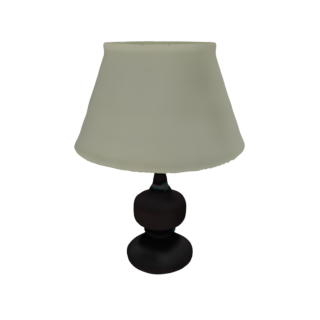
\includegraphics[width=0.15\linewidth, trim=70 45 70 40, clip]
{images/editings/shap-editor/lamps/shap_e/original_shap_e_tile_0.png} &
                        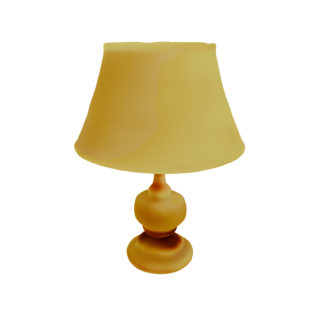
\includegraphics[width=0.15\linewidth, trim=70 45 70 40, clip]
{images/editings/shap-editor/lamps/edit1_shap_e/golden_shap_e_tile_0.png} &
                       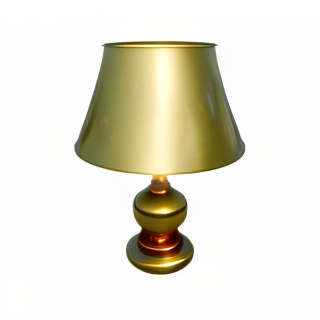
\includegraphics[width=0.15\linewidth, trim=70 45 70 40, clip]
{images/editings/shap-editor/lamps/edit1_sharp_e/0_75_steps_batch_0_a_golden_table_lamp_tile_0.png} \\
        %
        %
        & \multicolumn{4}{c}{``A table lamp'' $\longrightarrow$ ``A santa table lamp''} \\
        %
         &
                       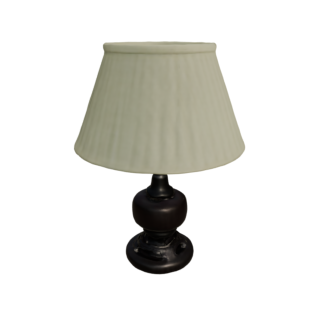
\includegraphics[width=0.15\linewidth, trim=70 45 70 40, clip]
{images/editings/shap-editor/lamps/original/render_0000.png} &
                      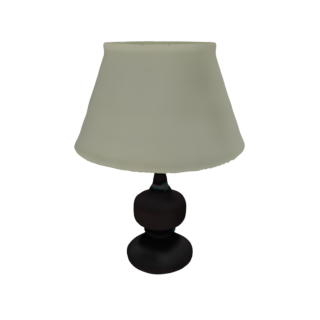
\includegraphics[width=0.15\linewidth, trim=70 45 70 40, clip]
{images/editings/shap-editor/lamps/shap_e/original_shap_e_tile_0.png} &
                    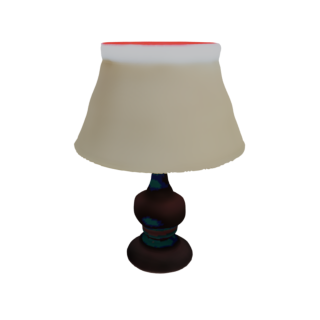
\includegraphics[width=0.15\linewidth, trim=70 45 70 40, clip]
{images/editings/shap-editor/lamps/edit2_shap_e/santa_0.png} &
                      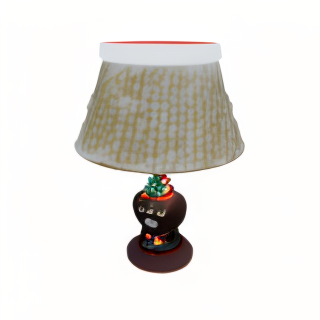
\includegraphics[width=0.15\linewidth, trim=70 45 70 40, clip]
{images/editings/shap-editor/lamps/edit2_sharp_e/0_75_steps_batch_0_a_santa_table_lamp_tile_0.png} \\
        %
        %
        & \multicolumn{4}{c}{``A blue beetle car'' $\longrightarrow$ ``A torquoise beetle car''} \\
        %
                        % L B R T

        \raisebox{12pt}{\multirow{3}{*}{\rotatebox[origin=t]{90}{DDPM Inversion}}} &
    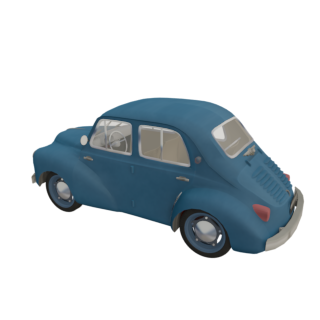
\includegraphics[width=0.22\linewidth, trim=30 60 15 85, clip]
{images/editings/ddpm_inv/original/render_0000.png} &
           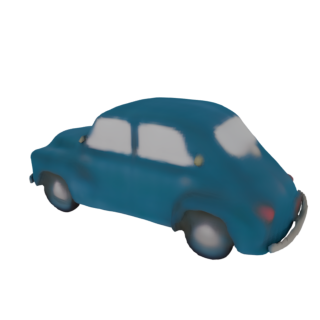
\includegraphics[width=0.22\linewidth, trim=30 60 15 85, clip]{images/editings/ddpm_inv/shap_e/original_shap_e_tile_0.png} &
           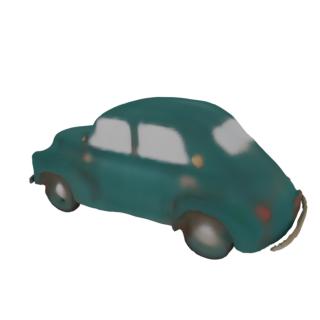
\includegraphics[width=0.22\linewidth, trim=30 60 0 85, clip]{images/editings/ddpm_inv/edit1_shap_e/torquoise_shap_e_tile_0.png} &
           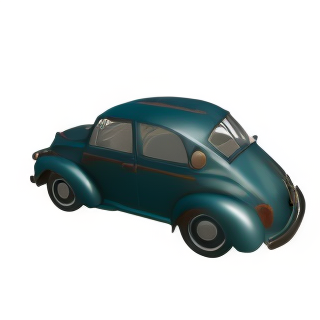
\includegraphics[width=0.22\linewidth, trim=30 60 0 85, clip]{images/editings/ddpm_inv/edit1_sharp_e/torquoise_beetle_car_75_steps_batch_0_a_matte_torquoise_beetle_car_tile_0.png} \\
        %
        %
         & \multicolumn{4}{c}{``A blue beetle car'' $\longrightarrow$ ``A blue SUV''} \\
        %
         &
             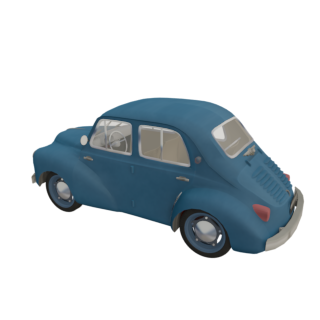
\includegraphics[width=0.22\linewidth, trim=30 60 15 85, clip]{images/editings/ddpm_inv/original/render_0000.png} &
            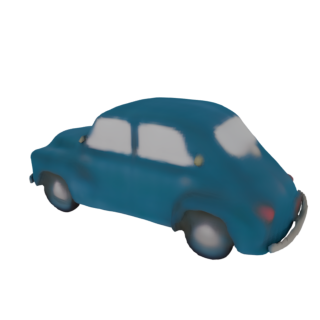
\includegraphics[width=0.22\linewidth, trim=30 60 15 85, clip]{images/editings/ddpm_inv/shap_e/original_shap_e_tile_0.png} &
           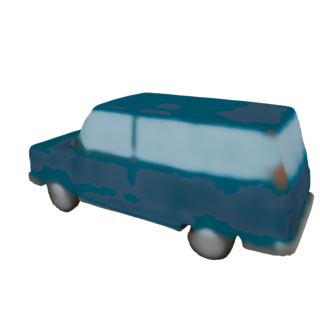
\includegraphics[width=0.22\linewidth, trim=30 60 0 85, clip]{images/editings/ddpm_inv/edit2_shap_e/mv_0_image_tile_0.png} &
               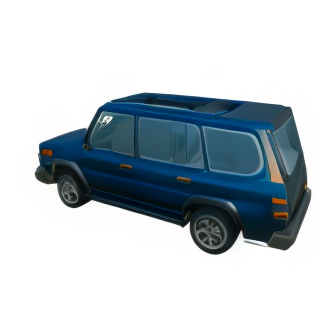
\includegraphics[width=0.22\linewidth, trim=30 60 0 85, clip]{images/editings/ddpm_inv/edit2_sharp_e/blue_suv_75_steps_batch_0_a_metalic_blue_suv_tile_0.png} \\
        %
        %
        & Input Shape & Encoded Shaped & Edit & + \ourname{}
    \end{tabular}
    }
    \vspace{-4pt}
    \caption{
    Our method enhances edits performed in Shap-E's space (rightmost column). We show editing results obtained with an existing editing method (Shap-Editor), and demonstrate that DDPM Inversion, originally developed for image diffusion models, works with Shap-E and can be integrated with \ourname{}.
    }
    \vspace{-16pt}
    \label{fig:edits}
\end{figure}